\section*{解答}
\subsection{第七章}
\begin{ans}
AからBへ向かうベクトルをAB,AからCへ向かうベクトルをACとすると,
\[\text{AB}=\begin{pmatrix} 3 \\ 3 \\ 3\end{pmatrix},\quad \text{AC}=\begin{pmatrix} 6 \\ 6 \\ 6\end{pmatrix}=2\text{AB}\]
このとき,$2\text{AB}-\text{AC}=\bm{0}$より,ABとACは線形従属であるため平行である.さらにどちらもAを通っているため,ABとACは同一直線上にある.よって,A,B,Cは同一直線上にある.
\end{ans}

\begin{ans}
$\bm{w}=\begin{pmatrix} w_1 \\ w_2 \\ w_3\end{pmatrix}\ (w_1\neq0,\ w_2\neq0,\ w_3\neq0)$とする.$\bm{u}$は$\bm{w}$と直交するので,
\begin{align*}
\bm{u}\cdot\bm{w}&=0\\
w_1+2w_2-w_3&=0
\end{align*}
$\bm{v}$は$\bm{w}$と直交するので,
\begin{align*}
\bm{v}\cdot\bm{w}&=0\\
3w_1-w_2+2w_3&=0
\end{align*}
よって,$w_1=-\dfrac{3}{7}w_3,\ w_2=\dfrac{5}{7}w_3$なので,$\bm{w}=\begin{pmatrix} -3 \\ 5 \\ 7\end{pmatrix}w_3\ (w_3\neq0)$.従って求める$\bm{w}$の一つは$\begin{pmatrix} -3 \\ 5 \\ 7\end{pmatrix}$.
\end{ans}

\begin{ans}
$\bm{A}=\begin{pmatrix} 1 & 1 \\ -1 & -1\end{pmatrix}$とすると,
\[\bm{A}^2=\begin{pmatrix} 1 & 1 \\ -1 & -1\end{pmatrix}\begin{pmatrix} 1 & 1 \\ -1 & -1\end{pmatrix}=\begin{pmatrix} 0 & 0 \\ 0 & 0\end{pmatrix}=\bm{O}\]
となる.
\end{ans}

\begin{ans}
$n+1$個以上のベクトルは余分なベクトルが含まれていて必ず線形従属になってしまう.逆に$n-1$個以下のベクトルでは$\mathbb{R}^n$のすべてのベクトルを線形結合で表すことができない.よって基底は$n$個である.
\end{ans}

\begin{ans}
$c_1\bm{v_1}+c_2\bm{v_2}+c_3\bm{v_3}=\bm{0}\ (c_1,\ c_2,\ c_3\in\mathbb{R})$とすると,
\[
\begin{pmatrix}
	c_1 + c_3\\
	c_2 + c_3\\
	c_1 + c_2
\end{pmatrix}
=
\begin{pmatrix}
	0\\
	0\\
	0
\end{pmatrix}
\]
より,$c_1=c_2=c_3=0$.よって,$\{\bm{v_1},\bm{v_2},\bm{v_3}\}$は線形独立.さらに,任意の$\begin{pmatrix} x\\ y\\ z \end{pmatrix}\in\mathbb{R}^3$に対して,
\[\begin{pmatrix} x\\ y\\ z \end{pmatrix}=\left(\frac{1}{2}x-\frac{1}{2}y+\frac{1}{2}z\right)\bm{v_1}+\left(-\frac{1}{2}x+\frac{1}{2}y+\frac{1}{2}z\right)\bm{v_2}+\left(\frac{1}{2}x+\frac{1}{2}y-\frac{1}{2}z\right)\bm{v_3}\]
と表せるので,$\{\bm{v_1},\bm{v_2},\bm{v_3}\}$は$\mathbb{R}^3$を生成する.よって,$\{\bm{v_1},\bm{v_2},\bm{v_3}\}$は$\mathbb{R}^3$の基底である.
\[
\bm{x}=\begin{pmatrix} 2\\ 3\\ 4 \end{pmatrix}=\frac{3}{2}\bm{v_1}+\frac{5}{2}\bm{v_2}+\frac{1}{2}\bm{v_3}
\]
\end{ans}

\begin{ans}
\begin{align*}
T\begin{pmatrix}1 \\ 0\end{pmatrix} &= \begin{pmatrix}\frac{1}{\sqrt{2}} \\ \frac{1}{\sqrt{2}}\end{pmatrix} = \frac{1}{\sqrt{2}}\begin{pmatrix}1 \\ 0\end{pmatrix} + \frac{1}{\sqrt{2}}\begin{pmatrix}0 \\ 1\end{pmatrix}\\
T\begin{pmatrix}0 \\ 1\end{pmatrix} &= \begin{pmatrix}-\frac{1}{\sqrt{2}} \\ \frac{1}{\sqrt{2}}\end{pmatrix} = -\frac{1}{\sqrt{2}}\begin{pmatrix}1 \\ 0\end{pmatrix} + \frac{1}{\sqrt{2}}\begin{pmatrix}0 \\ 1\end{pmatrix}
\end{align*}
よって表現行列は
\[\begin{pmatrix}\frac{1}{\sqrt{2}} & -\frac{1}{\sqrt{2}} \\ \frac{1}{\sqrt{2}} & \frac{1}{\sqrt{2}}\end{pmatrix}\]
\end{ans}

\begin{ans}
$\bm{A}+\bm{B}=\begin{pmatrix}0 & 2 \\ 5 & 5\end{pmatrix},\ \bm{A}-\bm{B}=\begin{pmatrix}2 & 2 \\ 1 & 3\end{pmatrix}$より,
\[(\bm{A}+\bm{B})(\bm{A}-\bm{B})=\begin{pmatrix}2 & 6 \\ 15 & 25\end{pmatrix}\]
$\bm{A}^2=\begin{pmatrix}7 & 10 \\ 15 & 22\end{pmatrix},\ \bm{A}-\bm{B}=\begin{pmatrix}1 & 0 \\ 0 & 1\end{pmatrix}$より,
\[\bm{A}^2-\bm{B}^2=\begin{pmatrix}6 & 10 \\ 15 & 21\end{pmatrix}\]
より確かに$(\bm{A}+\bm{B})(\bm{A}-\bm{B})\neq\bm{A}^2-\bm{B}^2$.\\
行列の積では一般に$\bm{A}\bm{B}\neq\bm{B}\bm{A}$なので,$(\bm{A}+\bm{B})(\bm{A}-\bm{B})=\bm{A}^2-\bm{A}\bm{B}+\bm{B}\bm{A}-\bm{B}^2$であるが,$-\bm{A}\bm{B}+\bm{B}\bm{A}=\bm{O}$とはならない.
\end{ans}

\begin{ans}
$\begin{pmatrix}1 \\ 2 \\ 1\end{pmatrix}=\begin{pmatrix}1 \\ 1 \\ 0\end{pmatrix}+\begin{pmatrix}0 \\ 1 \\ 1\end{pmatrix}$であるため,$\left\{\begin{pmatrix}1 \\ 1 \\ 0\end{pmatrix},\ \begin{pmatrix}0 \\ 1 \\ 1\end{pmatrix},\ \begin{pmatrix}1 \\ 2 \\ 1\end{pmatrix}\right\}$は線形従属である.また,$c_1\begin{pmatrix}1 \\ 1 \\ 0\end{pmatrix}+c_2\begin{pmatrix}1 \\ 0 \\ 1\end{pmatrix}=\bm{0}\ (c_1,\ c_2\in\mathbb{R})$とすると,$c_1=c_2=0$.よって,$\left\{\begin{pmatrix}1 \\ 1 \\ 0\end{pmatrix},\ \begin{pmatrix}0 \\ 1 \\ 1\end{pmatrix}\right\}$は線形独立.これらのことから,
\begin{align*}
V&=\text{span}\left\{\begin{pmatrix}1 \\ 1 \\ 0\end{pmatrix},\ \begin{pmatrix}0 \\ 1 \\ 1\end{pmatrix},\ \begin{pmatrix}1 \\ 2 \\ 1\end{pmatrix}\right\}=\text{span}\left\{\begin{pmatrix}1 \\ 1 \\ 0\end{pmatrix},\ \begin{pmatrix}0 \\ 1 \\ 1\end{pmatrix}\right\}\\
\dim(V)&=2
\end{align*}
基底の一つは$\left\{\begin{pmatrix}1 \\ 1 \\ 0\end{pmatrix},\ \begin{pmatrix}0 \\ 1 \\ 1\end{pmatrix}\right\}$.
\end{ans}

\begin{ans}
\begin{align*}
f\begin{pmatrix}1 \\ 0\end{pmatrix} &= \begin{pmatrix}1 \\ 2 \\ 1\end{pmatrix} = \begin{pmatrix}1 \\ 0 \\ 0\end{pmatrix} + 2\begin{pmatrix}0 \\ 1 \\ 0\end{pmatrix} + \begin{pmatrix}0 \\ 0 \\ 1\end{pmatrix}\\
f\begin{pmatrix}0 \\ 1\end{pmatrix} &= \begin{pmatrix}-1 \\ 0 \\ 1\end{pmatrix} = -\begin{pmatrix}1 \\ 0 \\ 0\end{pmatrix} + 0\begin{pmatrix}0 \\ 1 \\ 0\end{pmatrix} + \begin{pmatrix}0 \\ 0 \\ 1\end{pmatrix}\\
\end{align*}
よって表現行列は
\[\begin{pmatrix}1 & -1 \\ 2 & 0 \\ 1 & 1\end{pmatrix}\]
\end{ans}

\begin{ans}
\begin{align*}
f\begin{pmatrix}0 \\ 0\end{pmatrix} &= A\begin{pmatrix}0 \\ 0\end{pmatrix} = \begin{pmatrix}0 \\ 0\end{pmatrix}&
f\begin{pmatrix}1 \\ 0\end{pmatrix} &= A\begin{pmatrix}1 \\ 0\end{pmatrix} = \begin{pmatrix}1 \\ 0\end{pmatrix}\\
f\begin{pmatrix}0 \\ 1\end{pmatrix} &= A\begin{pmatrix}0 \\ 1\end{pmatrix} = \begin{pmatrix}1 \\ 1\end{pmatrix}&
f\begin{pmatrix}1 \\ 1\end{pmatrix} &= A\begin{pmatrix}1 \\ 1\end{pmatrix} = \begin{pmatrix}2 \\ 1\end{pmatrix}
\end{align*}
より下図となる.
\begin{center}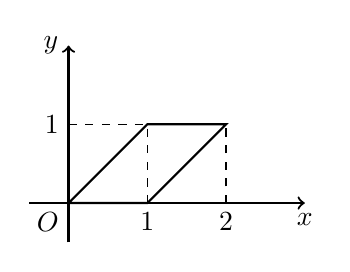
\begin{tikzpicture}
	\coordinate (O) at (0,0) node at (O) [below left] {$O$};
	\draw[thick, ->] (-0.5,0) -- (3,0) node [below] {$x$};
	\draw[thick, ->] (0,-0.5) -- (0,2) node [left] {$y$};
	\draw[thick] (O) -- (1, 1) -- (2,1) -- (1,0) -- (O);
	\draw[dashed] (0,1) -- (1, 1) -- (1, 0) (2, 0) -- (2, 1);
	\node at (1,0) [below] {1};
	\node at (2,0) [below] {2};
	\node at (0,1) [left] {1};
\end{tikzpicture}\end{center}
よって面積は$1\cdot1=1$.
\end{ans}